\chapter{Metodologia}
Este capítulo objetiva definir a metodologia que será utilizada na pesquisa, bem como apontar quais ferramentas serão usadas na
condução, coleta de dados e análise dos dados.  
\section{Caracterização do Estudo}
Aqui você deve dizer qual é o tipo de estudo realizado. Existem diversos autores propondo tipologias, por isso apresente a tipologia citando o autor de referência. Por exemplo: “A natureza de uma pesquisa está relacionada com seus objetivos gerais, sendo classicamente rotulada como exploratórias, descritivas ou explicativas (GIL, 1999).”.
Depois de apresentar as classificações dos metodologistas, aponte a que mais classifica a sua pesquisa, por exemplo: “Dessa forma, a presente pesquisa é de natureza descritiva”.
Classifique sua pesquisa também quanto às linhas gerais dos métodos de pesquisa a serem utilizados, ou seja, sua pesquisa será qualitativa, quantitativa ou mista? Lembre de antes mostrar como os metodologistas descrevem esses métodos.
Classifique também a estratégia de pesquisa a ser utilizada. Ex: “Existem diversas estratégias metodológicas de pesquisa, destacando-se as pesquisas documentais, os estudos de caso, as pesquisas-ação, os surveys, a prototipação, as pesquisas observacionais e os experimentos (LAKATOS; MARCONI, 2010). Para este estudo discorrer-se-á sobre as pesquisas observacionais, as pesquisas documentais e os estudos de caso por serem os que mais se ajustam ao objeto pesquisado.”.  
\section{Coleta de Dados}
Aqui você vai dizer como os dados serão coletados. Aproveite para esclarecer como foram selecionados seus respondentes, se for o caso. Diga também as etapas do seu trabalho.
\section{Análise de Dados}
Aqui você vai dizer como os dados serão analisados, lembrando de dizer o que os metodologistas explicam sobre cada técnica a ser utilizada.
\section{Desenho da pesquisa}
Para a conclusão dos objetivos propostos nesta pesquisa seram realizados algumas etapas as quais visão delinear este trabalho de forma sistematica a fim de garantir o direcionamento da mesma. 

A realização da pesquisa deste trabalho será embasada em experimentos, simulações e análises de dados, seguindo o fluxograma ilustrado na Figura~\ref{figpesquisa}. De forma mais direta, inicialmente a pesquisa constituirá de uma filtragem simplificada dos dados obtidos do grupo SXS, atraves de tecnicas de series temporais afim de trata-los e padronizar os dados para os experimentos. Existem diversas formas de analizar e filtrar dados de series temporais, mais comumente utilizadas como por exemplo os modelos:

\begin{figure}[ht]
\centering
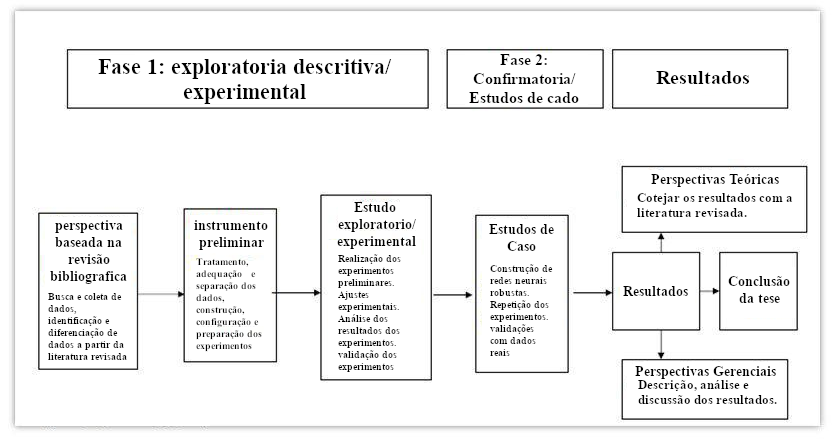
\includegraphics[width=1\textwidth]{figuras/desenho_da_pesquisa.png}
\caption{Desenho da pesquisa}
\label{figpesquisa}
\end{figure}

1 AR(p) → Modelo Auto-Regressivo de Ordem p;

2 MA(q) → Modelo Médias Móveis de Ordem q;

3 ARMA(p, q) → Modelo que combina AR(p) e MA(p);

4 ARIMA(p, d, q) → Modelo ARMA(p, q) com diferenciação de Ordem d.

Sendo que, em primeiro momento, não existirá a necessidade de se utilizar alguma dessas tecnicas de analises avançadas, em principio será utilizada somente uma normalização dos dados e uma previa separação de 3 niveis, em que, todas seram padronizadas com a retirada da sua derivada e somadas a uma variação de ruidos uniformes e galcianos que variam entre 10\% e 100\%.

Os niveis gerados após este tratamento de dados seram diferenciados pela janela de informação contida em cada um dos niveis, sendo que, cada um terá um decimo de informação do nivel anterior, ilustrado na Figura~\ref{figjanela}, começando com o nivel um, o qual, não tem nivel anterior e portanto terá uma janela de dados de 8192 pontos, seguido do segundo nivel, em que, tem uma janela de informação de 819 pontos e por ultimo o terceiro nivel que tem 82 pontos. As janelas de dados possuirão 10\% de sobreposição uma das outras, assim como mostra a Figura~\ref{figjanela}.

\begin{figure}[ht]
\centering
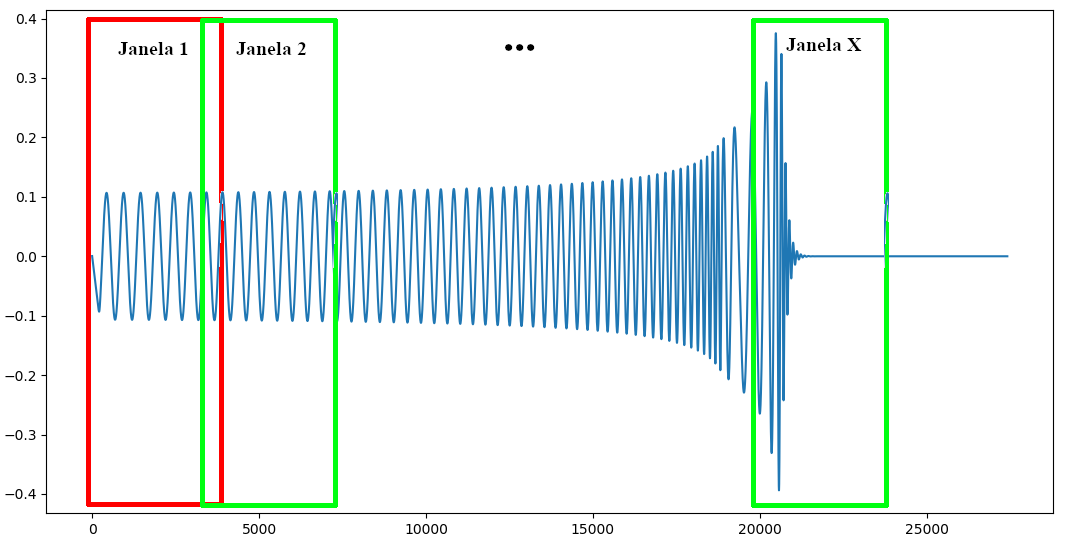
\includegraphics[width=1\textwidth]{figuras/janelas.png}
\caption{Janelas}
\label{figjanela}
\end{figure}

Para obter os resultados e respostas acerca da problematização apresentada neste trabalho, será montado um experimento com redes neurais artificiais do tipo perceptron, mais especificamente do tipo MultiLayerPerceptron, sendo o treinamento realizado atraves do metodo backpropagation, baseado no metodo de experimentação dos quadrados latinos, sem a necessiadade da analise estatistica, conforme é demostrado na Figura~\ref{figexperimento}. No experimento será feita a análise sobre a separabilidade do sinal de informalçao das ondas gravitacionais e o ruido atrelado a ele, será usado o teste Kolmogorov–Smirnov (também conhecido como teste KS ou teste K–S), o qual, será medido a distancia KS de cada um dos resultados do experimento, ilustrano na Figura~\ref{figkolmogorov}, afim de descobrir o nivel de separação das ondas gravitacionais do ruido.

\begin{figure}[ht]
\centering
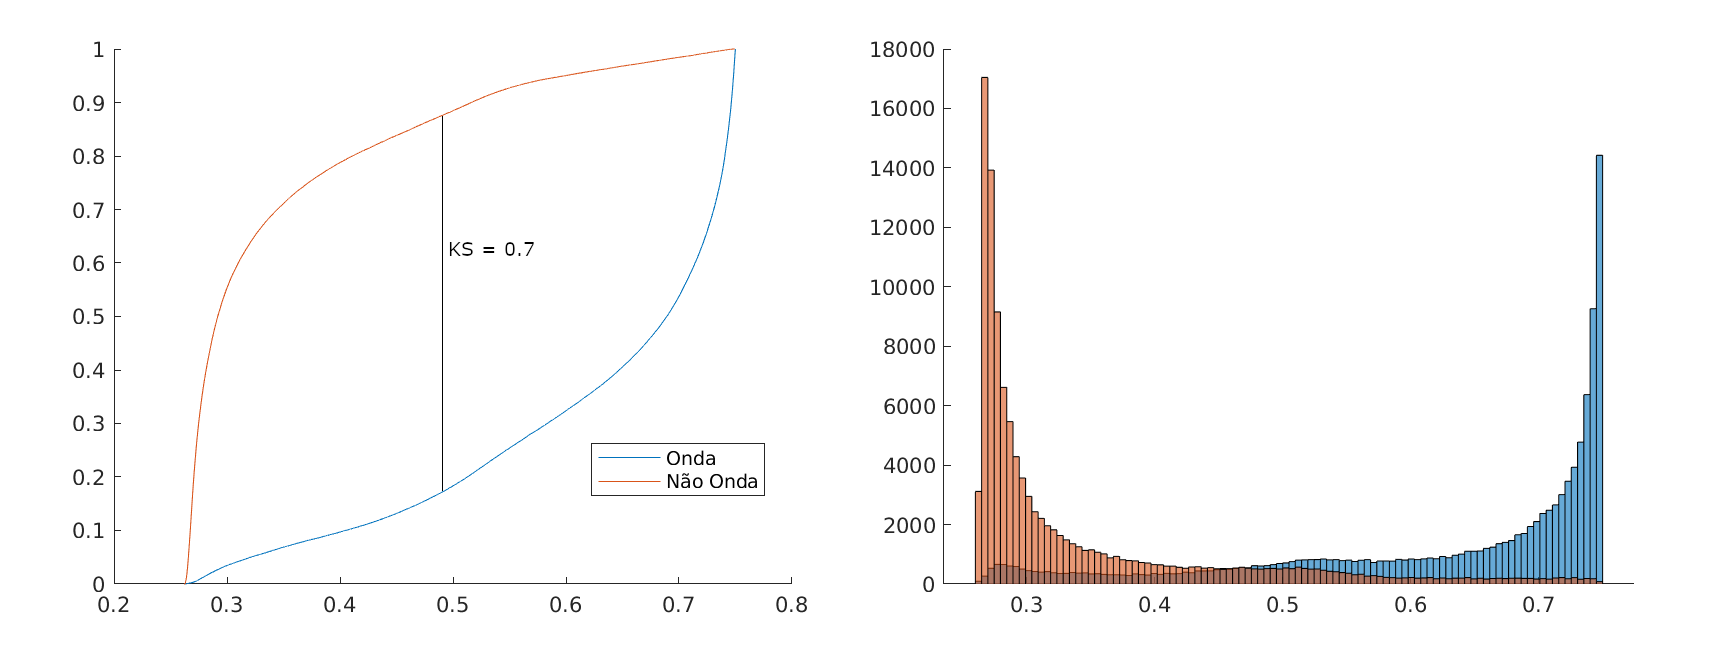
\includegraphics[width=1\textwidth]{figuras/test-kolmogorov.png}
\caption{Experimento}
\label{figkolmogorov}
\end{figure}

\begin{figure}[ht]
\centering
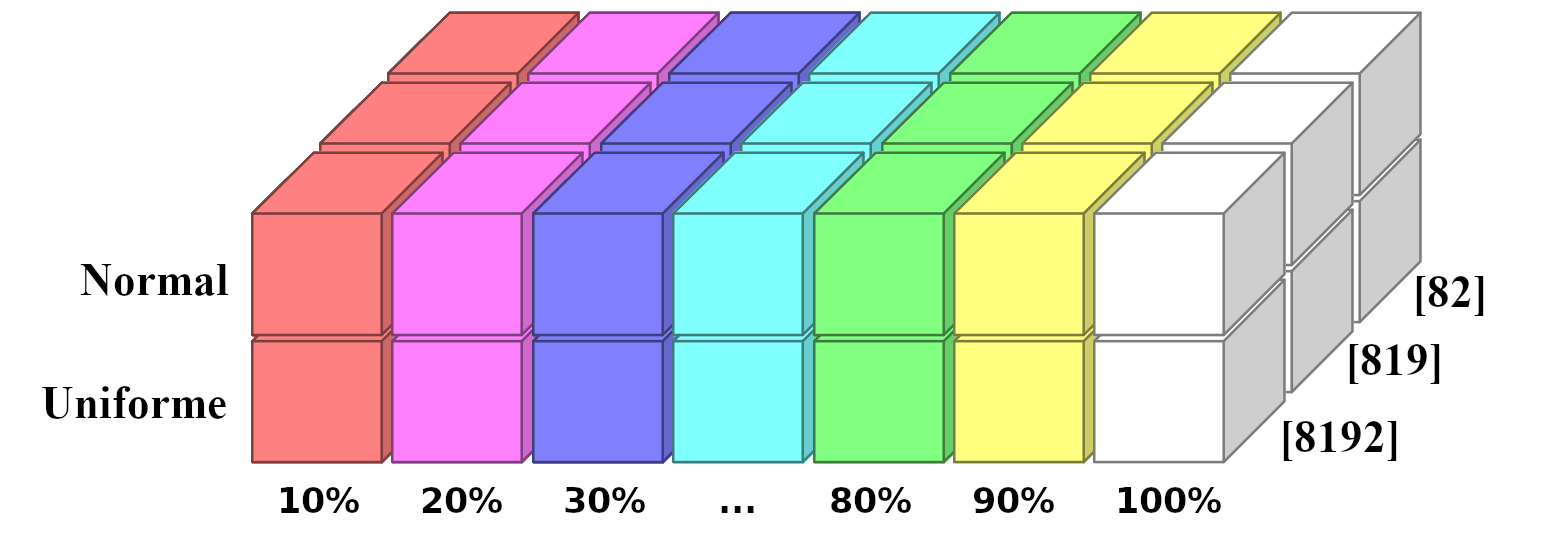
\includegraphics[width=1\textwidth]{figuras/experimento.png}
\caption{Experimento}
\label{figexperimento}
\end{figure}

A rede neural artificial que será usada terá somente duas camadas, sendo, uma de entrada e uma de saida, que contaram com 10 neuronios na primeira camada e 2 neuronios na segunda camada, conforme ilustrado na Figura XX. Como os dados foram separados em 3 niveis, em que, cada um tem uma janela de informações diferente, cada experimento se adequará a este tipo de janela, sendo assim, a rede neural artificial terá uma quantidade de entrada(input) diferente para cada experimento, o qual, mudará o nivel da janela de informação.

Após os resultados do primeiro experimento, sucederá uma nova etapa na pesquisa cujo delineamento dar-se-á para testes computacionais com diferentes abordagens de redes neurais artificiais, sendo elas, extreme learnign, Deep e Convulational. seguindo a mesma metodologia da primeira etapa desta pesquisa, desenrolar-se-á, os experimentos feitos anteriormente com abordagens de redes neurais artificiais diferentes para cada experimento, também calculando a distancia de Kolmogorov-Smirnov.

Logo depois de todos os experimentos serem feitos, haverá a necessidade de se fazer uma validação dos experimentos com os dados reais extraidos do LIGO, os quais, seram usados para validação dos experimentos e classificação dos resultados obtidos pelos mesmos.

E finalmente entraremos na etapa final, a qual, será para as analises dos resultados. Nesta analise haverá a necessidade de  se extrair todas as informações possiveis para se alcançar os objetivos desta pesquisa, para começar derá ser feita uma categorização de todos os KS obtidos atravez dos experimentos para então classificar a melhor rede e ao mesmo tempo determinar que tipo de ruido existe nos dados reais e em qual amplitide os compõem.

Os resultados obtidos pela analise final serão cotejados com os resultados da literatura revisada. Dado que se os resultados forem satisfatorios, sucederá a descrição, analise e discução dos resultados, afim de finalizar com a conclusão da escrita da disertação e a submissão de artigos para revistas e eventos, concluindo assim o mestrado.